\documentclass[12pt]{article}
\usepackage{graphicx}
\usepackage{hyperref}
\usepackage[top=2.75in, left=1in, right=1in, bottom=0.25in]{geometry}
\usepackage[utf8]{inputenc}
\usepackage[english]{babel}
\usepackage{fancyhdr}
\usepackage[utf8]{inputenc}
\usepackage{listings}
\usepackage{color}
\usepackage[final]{pdfpages}
\usepackage{multirow}
\usepackage{array}
\usepackage{caption}
\usepackage{subcaption}

\definecolor{codegreen}{rgb}{0,0.6,0}
\definecolor{codegray}{rgb}{0.5,0.5,0.5}
\definecolor{codepurple}{rgb}{0.58,0,0.82}
\definecolor{backcolour}{rgb}{0.95,0.95,0.92} 
\lstdefinestyle{mystyle}{
    backgroundcolor=\color{backcolour},   
    commentstyle=\color{codegreen},
    keywordstyle=\color{magenta},
    numberstyle=\tiny\color{codegray},
    stringstyle=\color{codepurple},
    basicstyle=\footnotesize,
    breakatwhitespace=false,         
    breaklines=true,                 
    captionpos=b,                    
    keepspaces=true,                 
    numbers=left,                    
    numbersep=5pt,                  
    showspaces=false,                
    showstringspaces=false,
    showtabs=false,                  
    tabsize=2
} 
\lstset{style=mystyle}

\setlength{\parindent}{4em}
\setlength{\parskip}{1em}
\pagestyle{fancy}
\fancyhf{}
\rhead{Assignment 10}
\lhead{Huan Huang}
\renewcommand{\headrulewidth}{0.4pt}
\renewcommand{\footrulewidth}{0.4pt}
\rfoot{Page \thepage}


\begin{document}
\begin{titlepage}
	\begin{center}
	\Huge{Web Science cs532-s16}\\
	[0.25in]
	\textsc{\Large Assignment 10 Report}\\
	\textsc{\normalsize Dr. Michael L. Nelson}\\
	[4.25in]
	\textsc{\normalsize By: Huan Huang}\\
	\large 04/30/2016\\
	
	
	\end{center}
\end{titlepage}
\newpage

\newgeometry{margin=1in}


\section*{Problem 1}


\begin{verbatim}
Using the data from A8:

- Consider each row in the blog-term matrix as a 500 dimension vector, 
corresponding to a blog.  

- From chapter 8, replace numpredict.euclidean() with cosine as the 
distance metric.  In other words, you'll be computing the cosine between
vectors of 500 dimensions.  

- Use knnestimate() to compute the nearest neighbors for both:

http://f-measure.blogspot.com/
http://ws-dl.blogspot.com/

for k={1,2,5,10,20}.
\end{verbatim}

\subsection*{Answer}
For this problem, I had some help from fellow classmate Ryan. Using data from assignment 8, I use the blog name ``F-Measure" and ``Web Science and Digital Libraries Research Group" to calculate the distance between these two blogs and every other blogs in the data file. It is done by calling function knnestimate(), which calls for getdistance() function. Getdistance() function will call for cosine() function to calculate distance between 2 vectors and return the result to knnestimate(). Knnestimate() then return the closest vectors based on the k values.



\begin{figure}[h!]
\centering
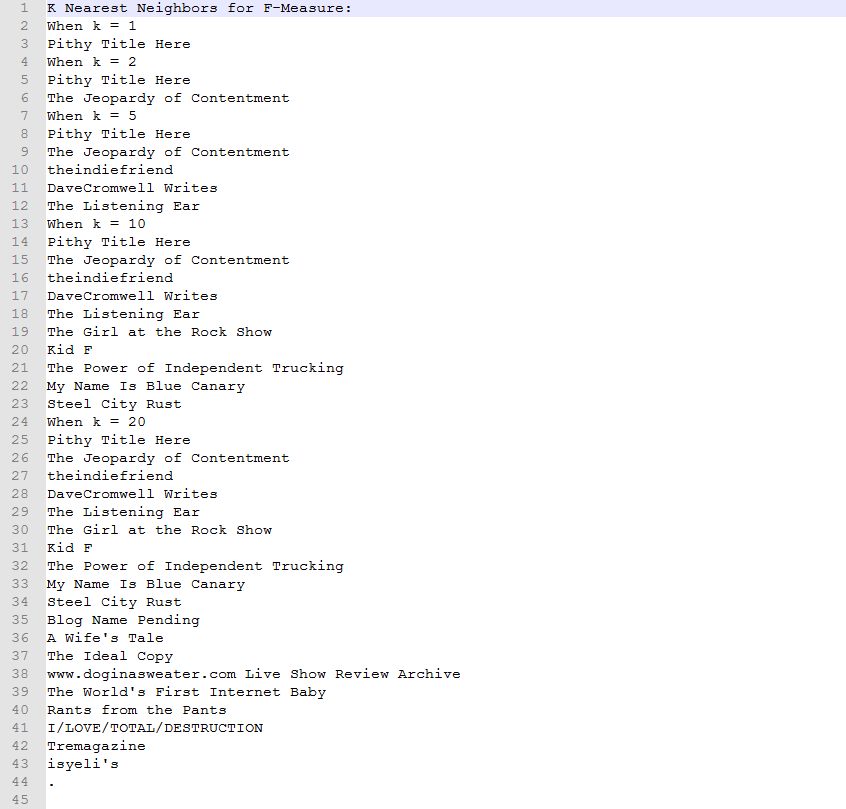
\includegraphics[width=6.5in]{KNNfmeasure.png}
\end{figure}
\newpage

\begin{figure}[h!]
\centering
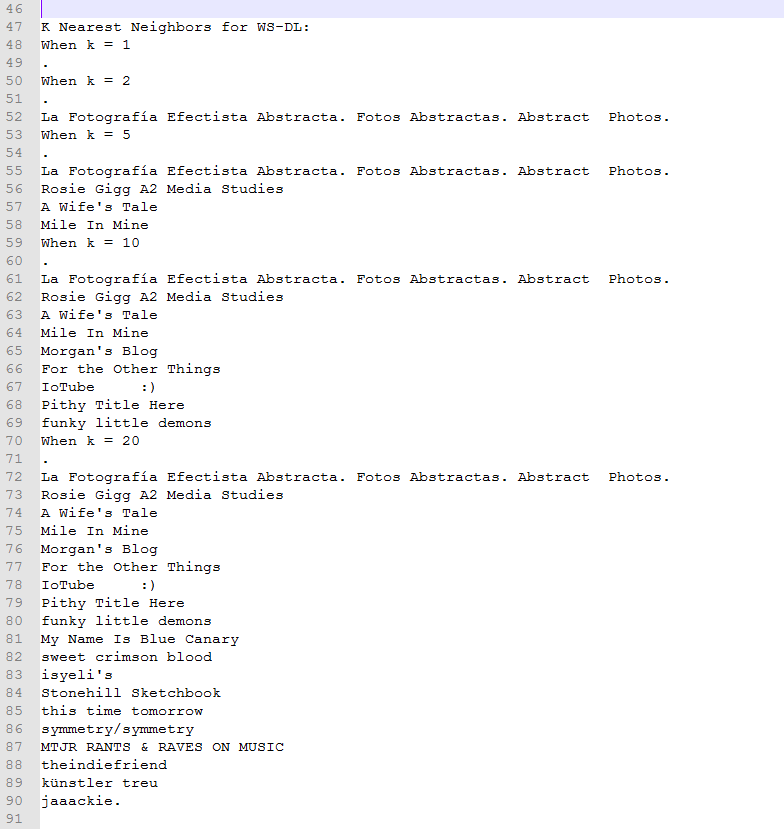
\includegraphics[width=6.5in]{KNNws_dl.png}
\end{figure}
\newpage

\lstinputlisting[language=python]{numpredict.py}

\section*{Problem 2}

\begin{verbatim}
Rerun A9, Q2 but this time using LIBSVM.  If you have n categories,
you'll have to run it n times.  For example, if you're classifying music
and have the categories:

metal, electronic, ambient, folk, hip-hop, pop

you'll have to classify things as:

metal / not-metal
electronic / not-electronic
ambient / not-ambient

etc.

Use the 500 term vectors describing each blog as the features, and
your mannally assigned classifications as the true values.  Use
10-fold cross-validation (as per slide 46, which shows 4-fold
cross-validation) and report the percentage correct for 
each of your categories.
\end{verbatim}

\subsection*{Answer}

\section*{Problem 3}
\begin{verbatim}
Re-download the 1000 TimeMaps from A2, Q2.  Create a graph where
the x-axis represents the 1000 TimeMaps.  If a TimeMap has "shrunk",
it will have a negative value below the x-axis corresponding to the
size difference between the two TimeMaps.  If it has stayed the
same, it will have a "0" value.  If it has grown, the value will be 
positive and correspond to the increase in size between the two
TimeMaps.

As always, upload all the TimeMap data.  If the A2 github has the 
original TimeMaps, then you can just point to where they are in 
the report.
\end{verbatim}
\subsection*{Answer}
To solve this problem, I downloaded the 1000 TimeMaps again and putted both the old memento count and new memento count into a spread sheet to do the calculation. To see the changes, I subtracted the old memento counts from the new memento counts. If the result of one subtraction is negative, then, this page has been removed from some archives. If the result is positive, then there are more archives of this web page. In my case, I do not have any negatives in my list of 1000 URIs. There are actually large amount of increment across the board. I used log scale in my y axis because of one URI that has very large amount of increment in memento counts than rest of them. All the TimeMap data are provided in folder Problem3 on my github account.

\begin{figure}[h!]
\centering
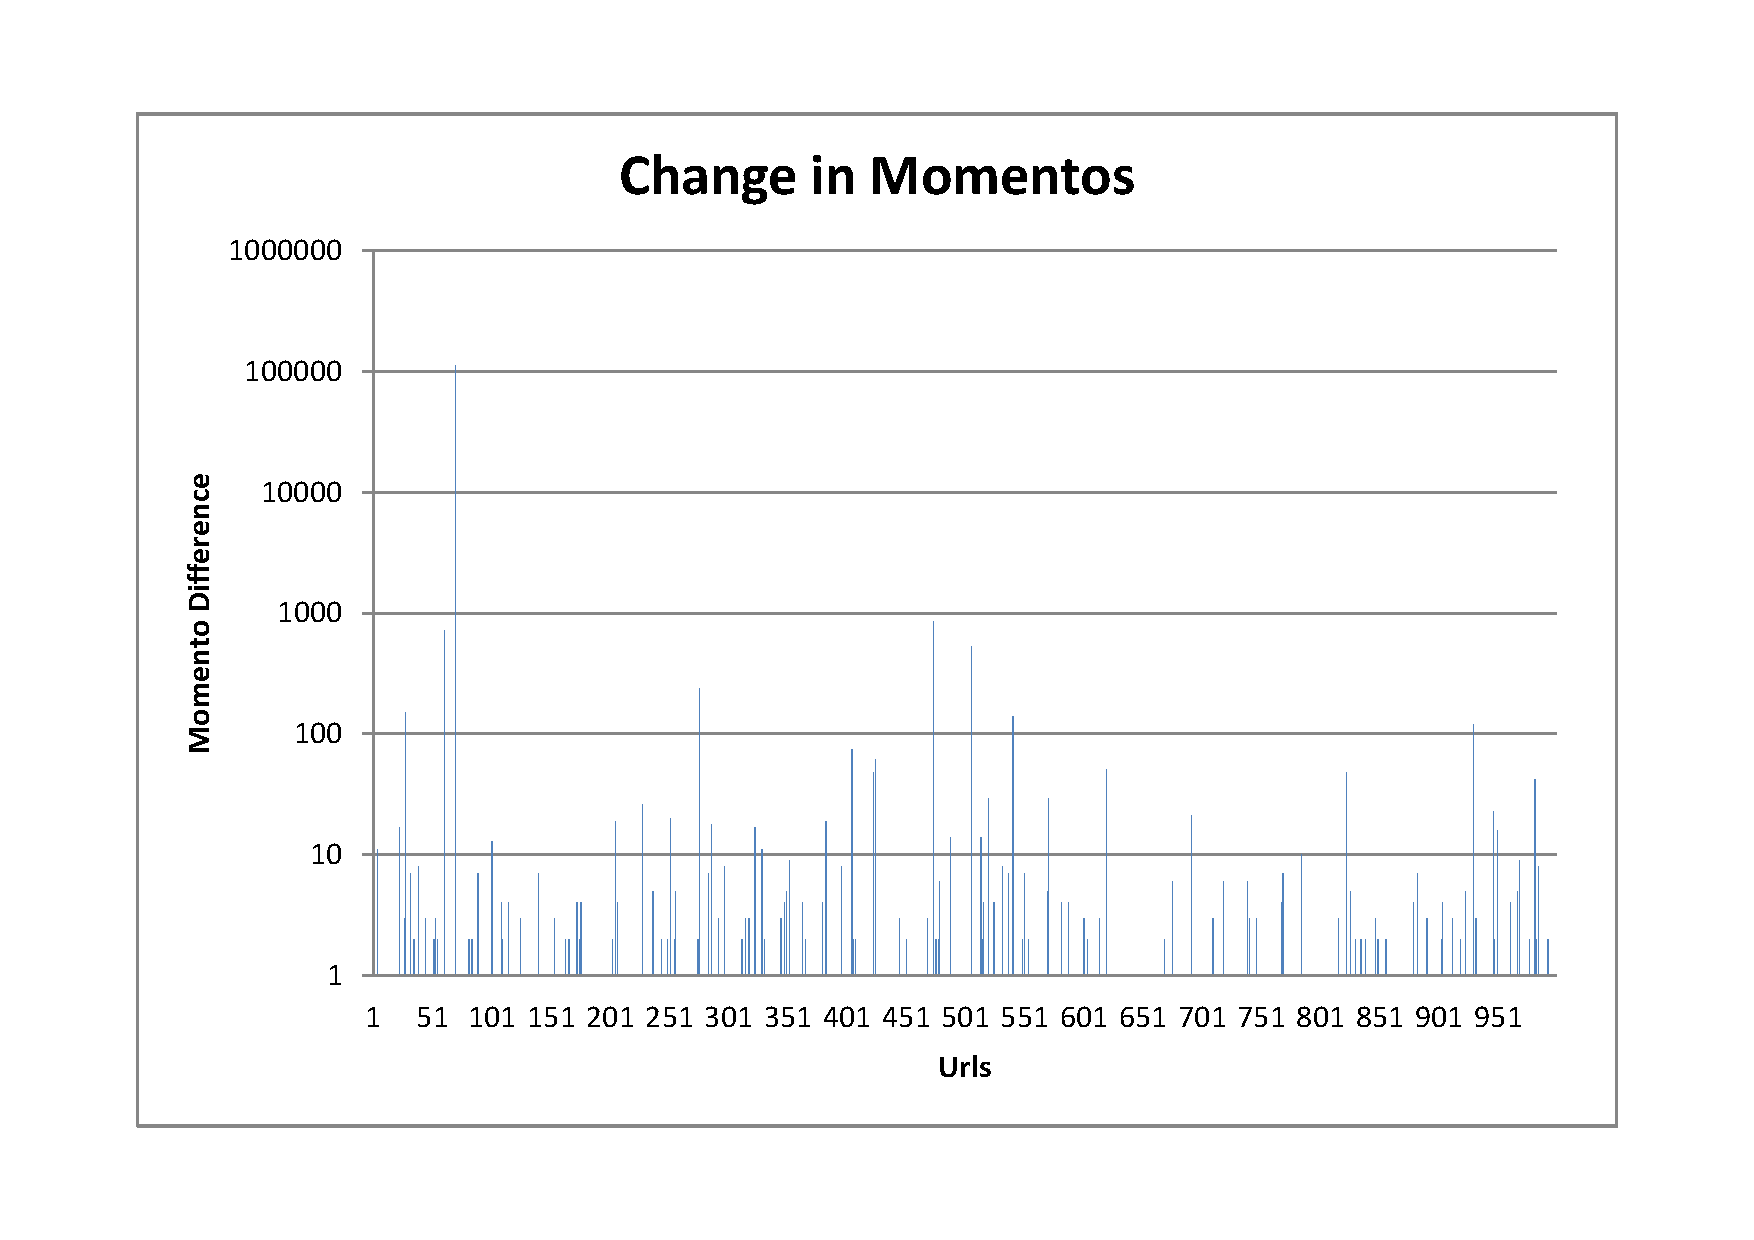
\includegraphics[width=6.5in]{difference.pdf}
\end{figure}

\begin{figure}[h!]
\centering
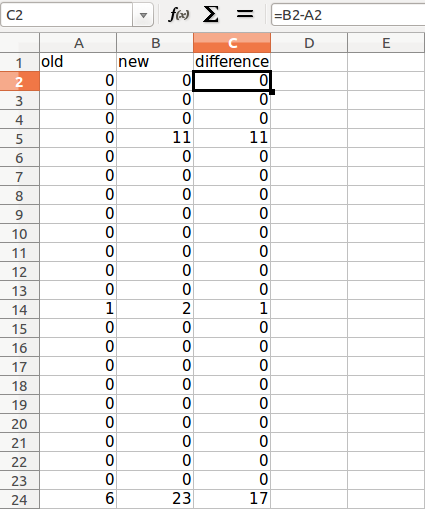
\includegraphics[width=5in]{difference.png}
\caption{Sample of newsubold.xlsx}
\end{figure}

\section*{Problem 4}
\begin{verbatim}
Repeat A3, Q1.  Compare the resulting text from February to 
the text you have now.  Do all 1000 URIs still return a "200 OK" 
as their final response (i.e., at the end of possible redirects)?

Create two graphs similar to that described in Q3, except this 
time the y-axis corresponds to difference in bytes (and not difference
in TimeMap magnitudes).  For the first graph, use the difference
in the raw (unprocessed) results.  For the second graph, use the 
difference in the processed (as per A3, Q1) results.

Of the URIs that still terminate in a "200 OK" response, pick the
top 3 most changed (processed) pairs of pages and use the Unix
"diff" command to explore the differences in the version pairs.
\end{verbatim}

\subsection*{Answer}
To solve this problem, I repeated the process in assignment 3 question 1. Then I wrote a piece of code to give me the file sizes of every old and new files. Then the results are put together in spread sheets to calculate the differences. All of the data and files are available in github.

\begin{figure}[h!]
\centering
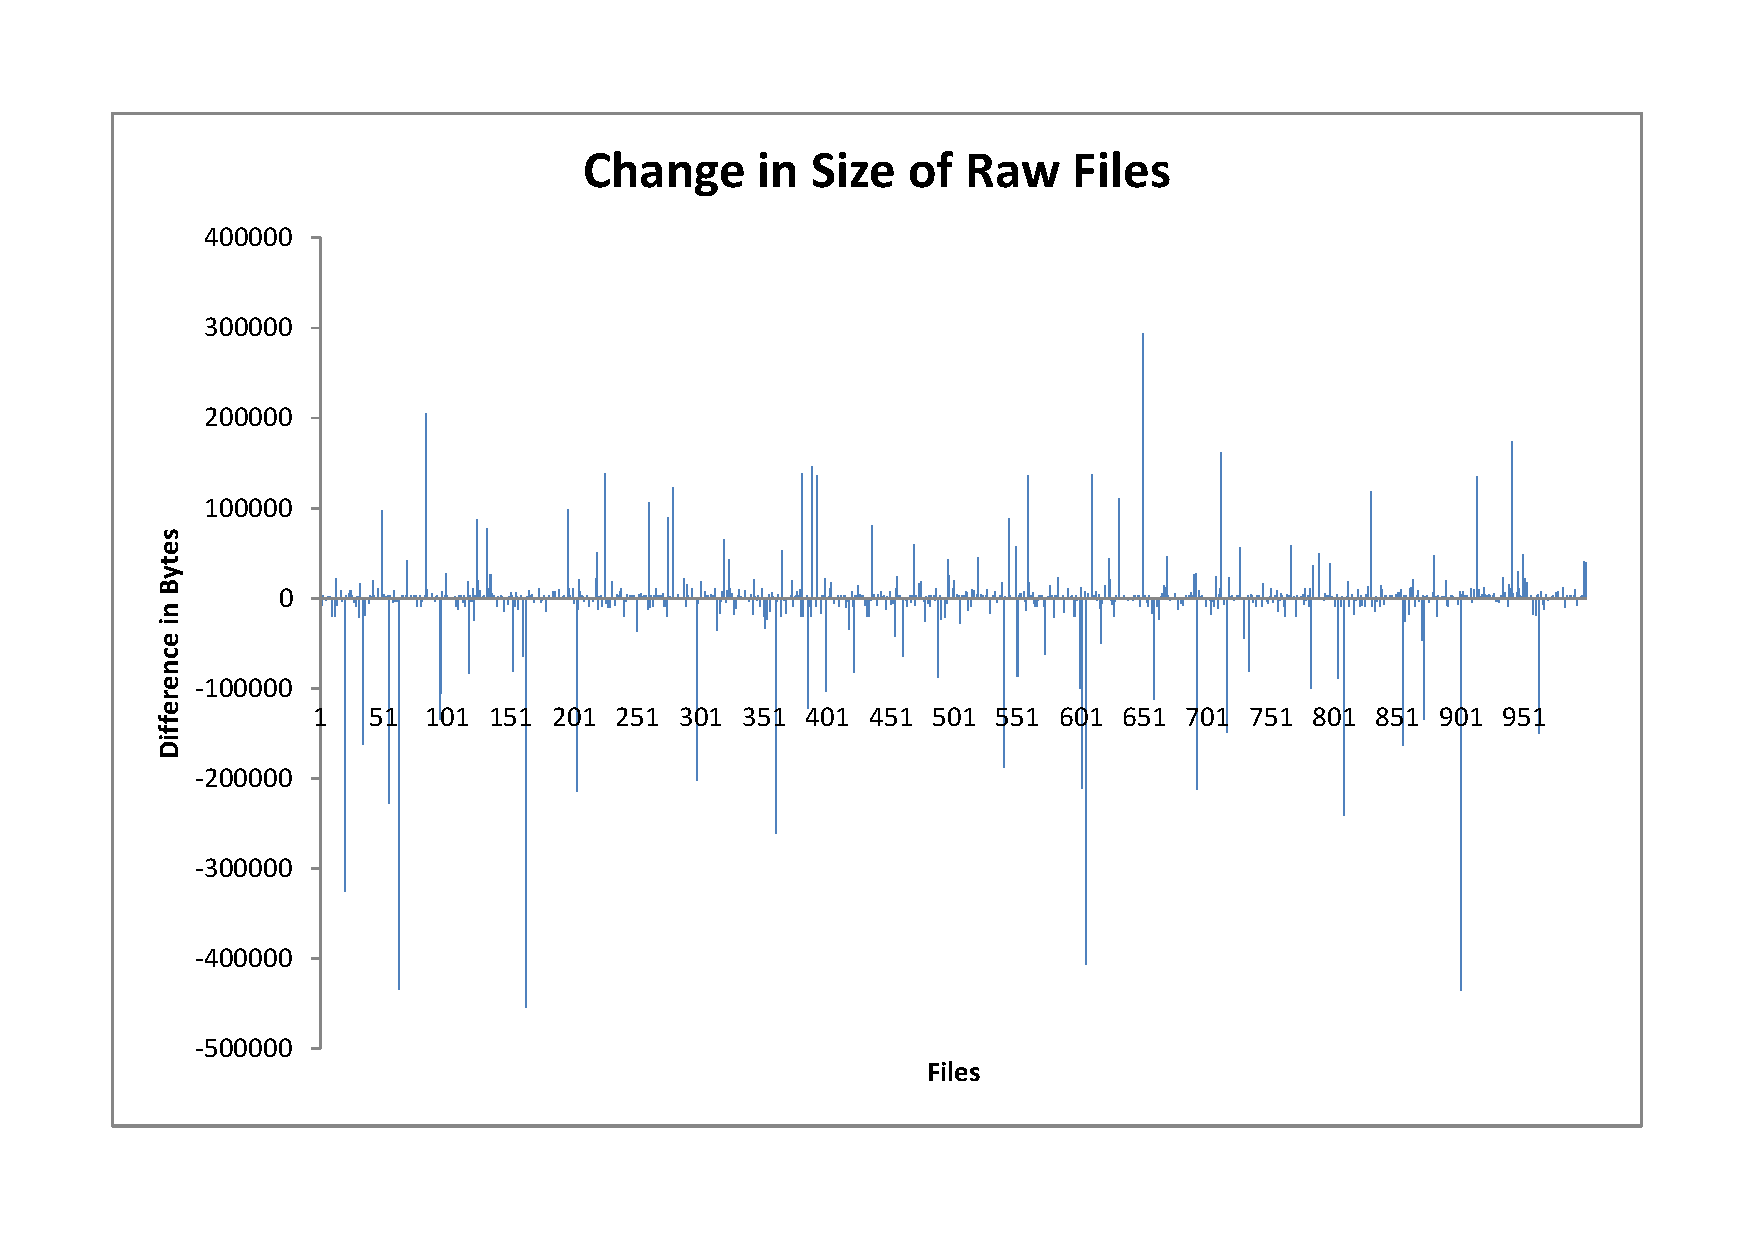
\includegraphics[width=6.5in]{RawDifference.pdf}
\end{figure}

In the processed files, between file 14.txt new and file 14.txt old, there is a huge amount of decrement in size comparing with other file size changes. Which made it hard to observe the graph accurately. 
\newpage

\begin{figure}[h!]
\centering
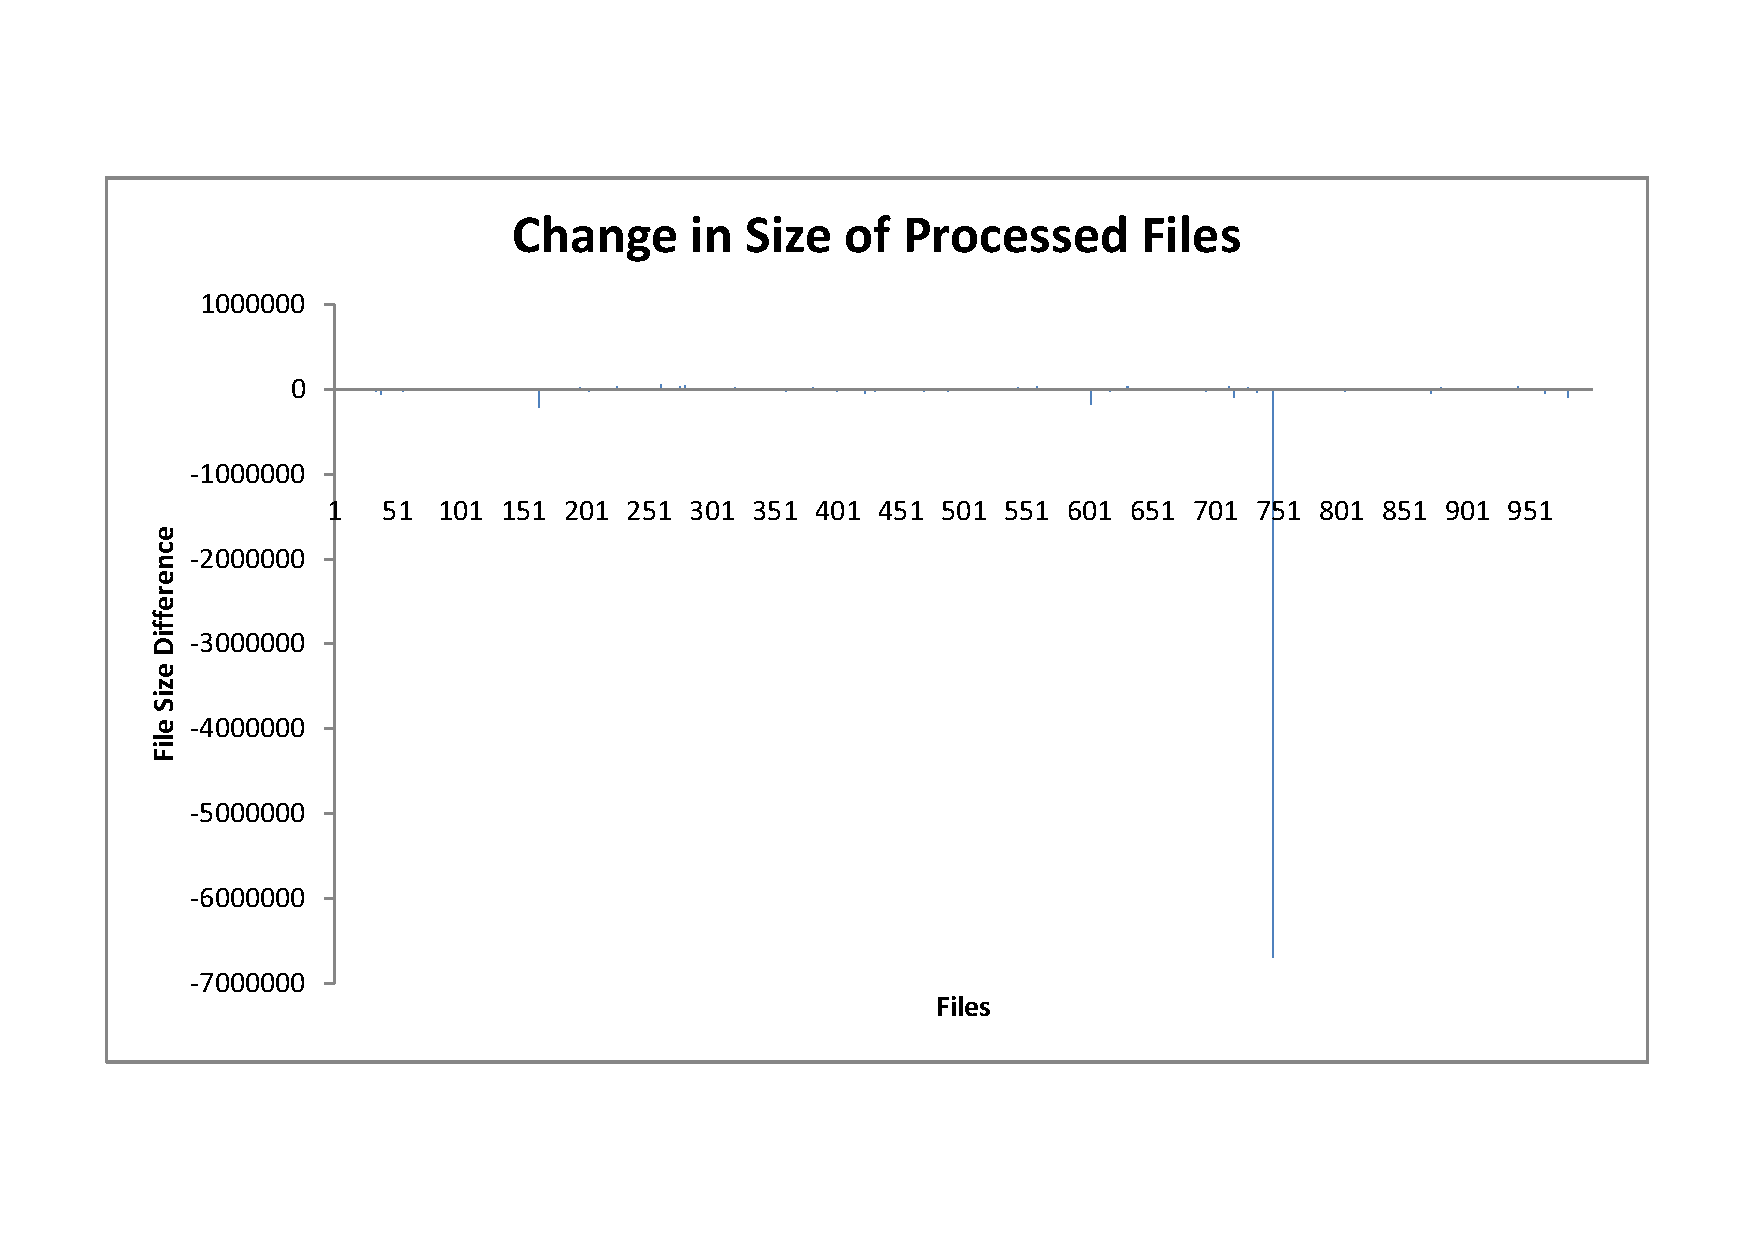
\includegraphics[width=6.5in]{ProcessedDifference.pdf}
\end{figure}

\lstinputlisting[language=python]{differenceSize.py}

I use command ``diff filename1 filename2" to get the differences of top 3 most changed pairs. The differences are saved in file names diff14.txt, diff276.txt, and diff571.txt. The files are too large to be shown in this report, they can be find in the ``3most" folder in Problem4 folder on my github account. 

\end{document}